\section{Caso ejemplo: cavidad cuadrada hidrodin\'amica}

\begin{frame}
    \frametitle{Estructura de archivos}
%    \framesubtitle{T\'ermino temporal}

    \begin{columns}
        
        \column{0.4\textwidth}
        \begin{figure}
            \centering
            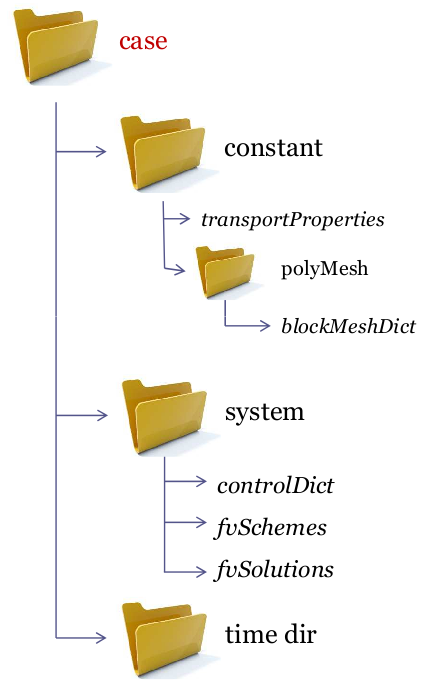
\includegraphics[scale=0.3]{Imagenes/file_structure_2}
        \end{figure}
        
        
        \column{0.5\textwidth}
        \footnotesize
        \begin{enumerate}
            \item {\bf 0} \\
                  Directorio de tiempo. Se almancenan las variables dependientes del problema.
            \begin{itemize}
                \tiny
                \item p
                \item U
            \end{itemize}
            
            \item {\bf constant} \\
                  Constantes del problema. Datos de la malla y propiedades f\'isicas.
            \begin{itemize}
                \tiny
                \item transportProperties: definici\'on de la viscosidad laminar
                \item blockMeshDict: diccionario para blockMesh (malla).
            \end{itemize} 
            
            \item {\bf system} \\
                  Discretizaci\'on, algoritmo y control de ejecuci\'on
            \begin{itemize}
                \tiny
                \item controlDict: paso de tiempo, intervalo de escritura, etc.
                \item fvSchemes: esquemas de discretizaci\'on.
                \item fvSolution: sistemas lineales, constantes para PISO/SIMPLE.
            \end{itemize} 
                       
        \end{enumerate}
        
    \end{columns}
    


\end{frame} 








\begin{frame}[fragile]
    \frametitle{Estructura de archivos}
    \framesubtitle{blockMeshDict}

\vspace{-0.8cm}
    \begin{columns}
        
        \column{0.4\textwidth}
            \begin{figure}
                \centering
                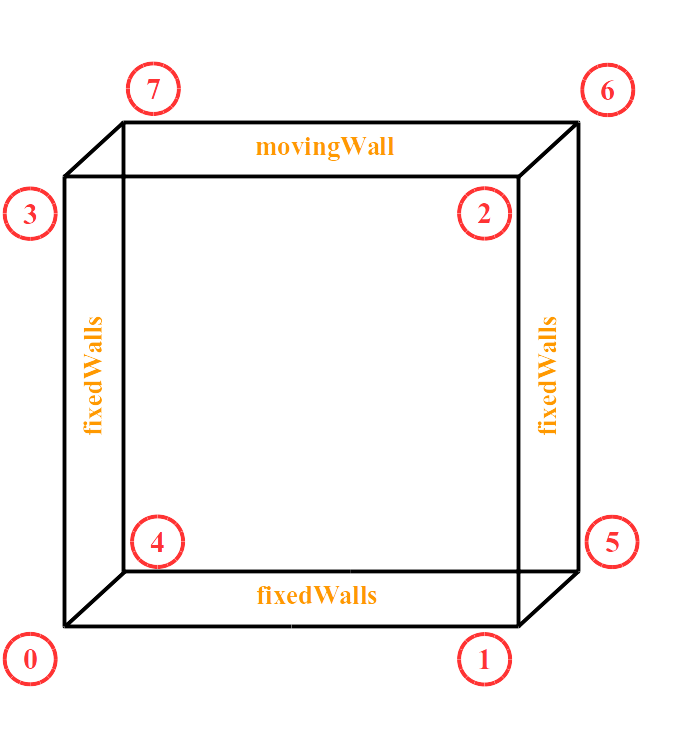
\includegraphics[scale=0.2]{Imagenes/Cavity/cavity_2}
            \end{figure}
\vspace{-0.8cm}            
            \tiny
            \begin{verbatim}
    vertices
    (
        (0 0 0)
        (1 0 0)
        (1 1 0)
        (0 1 0)
        (0 0 0.1)
        (1 0 0.1)
        (1 1 0.1)
        (0 1 0.1)
    );
              
    blocks
    (
        hex (0 1 2 3 4 5 6 7) (20 20 1) simpleGrading (1 1 1)
    );        
            \end{verbatim}
        
        
        \column{0.5\textwidth}
        \tiny
        \begin{verbatim}
                boundary
                (
                    movingWall
                    {
                        type wall;
                        faces
                        (
                            (3 7 6 2)
                        );
                    }
                    fixedWalls
                    {
                        type wall;
                        faces
                        (
                            (0 4 7 3)
                            (2 6 5 1)
                            (1 5 4 0)
                        );
                    }
                    frontAndBack
                    {
                        type empty;
                        faces
                        (
                            (0 3 2 1)
                            (4 5 6 7)
                        );
                    }
                );                    
        \end{verbatim}
        
    \end{columns}
    


\end{frame} 








\begin{frame}[fragile]
    \frametitle{Estructura de archivos}
    \framesubtitle{Variables dependientes}

\vspace{-0.8cm}
    \begin{columns}
        
        \column{0.45\textwidth}
            
            \begin{block}{\centering p}
        
            \tiny
            \begin{verbatim}

    dimensions      [0 2 -2 0 0 0 0];

    internalField   uniform 0;

    boundaryField
    {
        movingWall
        {
            type            zeroGradient;
        }

        fixedWalls
        {
            type            zeroGradient;
        }

        frontAndBack
        {
            type            empty;
        }
    }       
            \end{verbatim}                
            \end{block}

                
        \column{0.45\textwidth}
        
            \begin{block}{\centering U}

        \tiny
        \begin{verbatim}

    dimensions      [0 1 -1 0 0 0 0];

    internalField   uniform (0 0 0);

    boundaryField
    {
        movingWall
        {
            type            fixedValue;
            value           uniform (1 0 0);
        }

        fixedWalls
        {
            type            fixedValue;
            value           uniform (0 0 0);
        }

        frontAndBack
        {
            type            empty;
        }
    }                  
        \end{verbatim}
                
            \end{block}        

        
    \end{columns}
    


\end{frame} 







\begin{frame}[fragile]
    \frametitle{Estructura de archivos}
    \framesubtitle{fvSchemes}

\vspace{-0.8cm}
    \begin{columns}
        
        \column{0.4\textwidth}
            
            \begin{block}{\centering temporal}
        
            \tiny
            \begin{verbatim}
    ddtSchemes
    {
        default         Euler;
    }     
            \end{verbatim}                
            \end{block}


            \begin{block}{\centering gradiente}
        
            \tiny
            \begin{verbatim}
    gradSchemes
    {
        default         Gauss linear;
        grad(p)         Gauss linear;
    }
            \end{verbatim}                
            \end{block}
                
        \column{0.4\textwidth}
        
        \begin{block}{\centering convectivo}

        \tiny
        \begin{verbatim}
    divSchemes
    {
        default         none;
        div(phi,U)      Gauss linear;
    }
        \end{verbatim}
                
        \end{block} 
        
        
        
        \begin{block}{\centering difusivo}

        \tiny
        \begin{verbatim}
   laplacianSchemes
   {
       default   Gauss linear orthogonal;
   }
        \end{verbatim}
                
        \end{block}                

        
    \end{columns}
    


\end{frame} 








\begin{frame}[fragile]
    \frametitle{Estructura de archivos}
    \framesubtitle{fvSolution}

\vspace{-0.8cm}
    \begin{columns}
        
        \column{0.45\textwidth}
            
            \begin{block}{\centering Sistemas lineales}
        
            \tiny
            \begin{verbatim}
    solvers
    {
        p
        {
            solver          PCG;
            preconditioner  DIC;
            tolerance       1e-06;
            relTol          0;
        }

        U
        {
            solver          smothSolver;
            smoother        symGaussSeidel;
            tolerance       1e-05;
            relTol          0;
        }
    }      
            \end{verbatim}                
            \end{block}

                
        \column{0.45\textwidth}
        
            \begin{block}{\centering Algoritmo para N-S}

        \tiny
        \begin{verbatim}
    PISO
    {
        nCorrectors     2;
        nNonOrthogonalCorrectors 0;
        pRefCell        0;
        pRefValue       0;
    }                 
        \end{verbatim}
                
            \end{block}        

        
    \end{columns}
    


\end{frame} 






\begin{frame}[fragile]
    \frametitle{Estructura de archivos}
    \framesubtitle{controlDict}

\vspace{-0.8cm}
    \begin{columns}
        
        \column{0.45\textwidth}
            
            \begin{block}{}
        
            \footnotesize
            \begin{verbatim}
    application     icoFoam;

    startFrom       startTime;

    startTime       0;

    stopAt          endTime;

    endTime         0.5;

    deltaT          0.005;

    writeControl    timeStep;

    writeInterval   20;    
            \end{verbatim}                
            \end{block}

                
        \column{0.45\textwidth}
        
            \begin{block}{}

        \footnotesize
        \begin{verbatim}
    purgeWrite      0;

    writeFormat     ascii;

    writePrecision  6;

    writeCompression off;

    timeFormat      general;

    timePrecision   6;

    runTimeModifiable true;               
        \end{verbatim}
                
            \end{block}        

        
    \end{columns}
    


\end{frame} 






\begin{frame}[fragile]
    \frametitle{Ejecuci\'on}
%    \framesubtitle{E}
    \begin{columns}        
        \column{0.25\textwidth}
        \begin{enumerate}
            \item<1> blockMesh
            \item<2> icoFoam
            \item<3> paraFoam
        \end{enumerate}
        
        \column{0.65\textwidth}
        \begin{figure}
            \centering
            \includegraphics<1>[scale=0.3]{Imagenes/Cavity/mesh}
            \includegraphics<2>[scale=0.2]{Imagenes/Cavity/icoFoam}
            \includegraphics<3>[scale=0.4]{Imagenes/Cavity/U}
        \end{figure}


    \end{columns}        
    
\end{frame}     
